\documentclass{beamer}

\usepackage{amsmath}
\usepackage{amssymb}
\usepackage{latexsym}
\usepackage{textpos}
\usepackage[latin1]{inputenc}
\usepackage{multicol}
\usepackage{xcolor}

\usetheme{Warsaw}
\useinnertheme{default}
\useoutertheme{infolines}

%\mode<presentation> {
%   \setbeamercovered{transparent}
% }

\title[Algoritmos y Estructuras de Datos III]{Taller de Heur�sticas}

\institute[DC-FCEyN-UBA]{Departamento de Computaci\'on,\\Facultad de Ciencias Exactas y Naturales,\\Universidad de Buenos Aires}
\author{Iv�n Badgen}
\date{25 de Octubre de 2013}

\begin{document}

\frame{\titlepage}

%\begin{frame}{Contenido}
%\tableofcontents
%\end{frame}

\begin{frame}{Introducci�n}
 \begin{block}{�Qu� vamos a hacer?}
	Vamos a introducir un problema nuevo de optimizaci�n combinatoria, profundizarlo un poco, pensar heur�sticas e implementarlas.
  \end{block}
  \pause
   \begin{block}{�Vamos a competir!}
	Van a intercambiarse soluciones entre ustedes e intentar encontrar casos malos para los algoritmos desarrollados.
  \end{block}

\end{frame}

\begin{frame}{Conjunto dominante en grafos}
\begin{block}{Definici�n}
	Un conjunto dominante de un grafo $G$ $=$ $(V, E)$ es un conjunto de nodos $V^{'} \subseteq V$ tal que todo nodo de $V - V^{'}$ es adyacente
	a alg�n nodo de $V^{'}$.
\end{block} 
\pause
\begin{block}{Pregunta 1}
	�Es $V$ un conjunto dominante de G?
\end{block} 
\pause
\begin{block}{Problema de optimizaci�n}
	Dado un grafo $G$, el problema de m�nimo conjunto dominante consiste en encontrar un conjunto dominante de $G$ con la menor
	cantidad posible de nodos.
\end{block} 
\pause
\begin{block}{Pregunta 2}
	Dado un grafo $G$ cualquiera, �el m�nimo conjunto dominante ser� �nico?
\end{block} 
\end{frame}

\begin{frame}{Ejemplo}

Un grafo con tres de sus conjuntos dominantes. 

\begin{figure}
    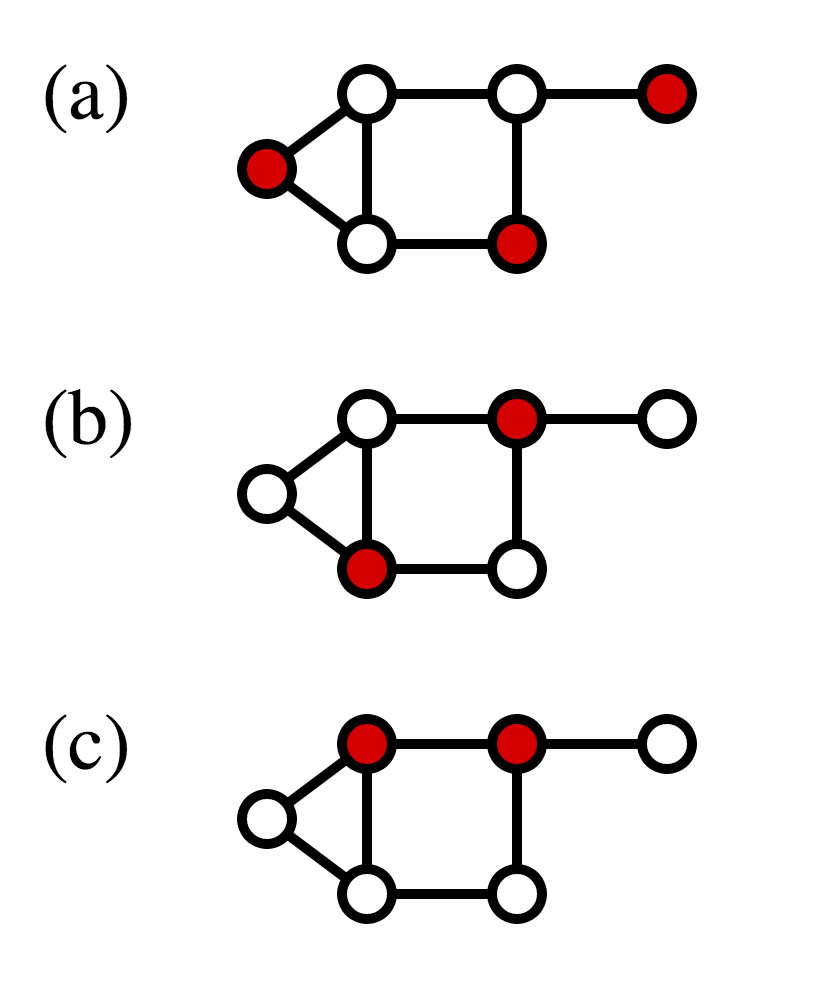
\includegraphics[scale=0.3]{img/dominating-set.png} 
  \end{figure}

\pause

�C�mo identificamos si un conjunto de dos nodos es �ptimo o podemos mejorarlo?

\end{frame}

\begin{frame}{Algunas familias}

\begin{block}{Estrellas }
	\begin{figure}
	    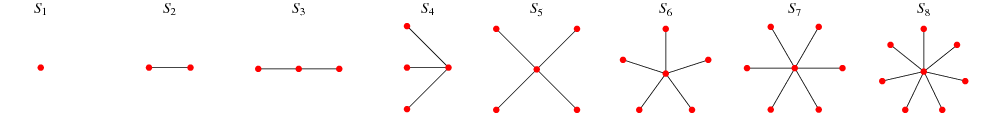
\includegraphics[scale=0.3]{img/star_graphs.png} 
	  \end{figure}
\end{block}
\pause
\begin{block}{Completos}
	\begin{figure}
	    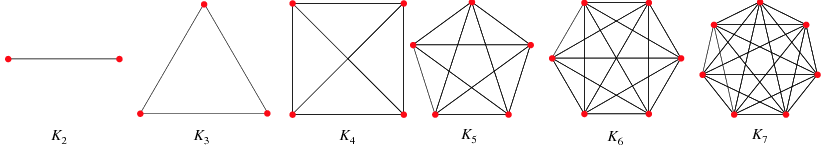
\includegraphics[scale=0.3]{img/complete_graphs.png} 
	  \end{figure}
\end{block}
\end{frame}

\begin{frame}{Algunas familias (2)}

\begin{block}{Disconexos }
	\begin{figure}
	    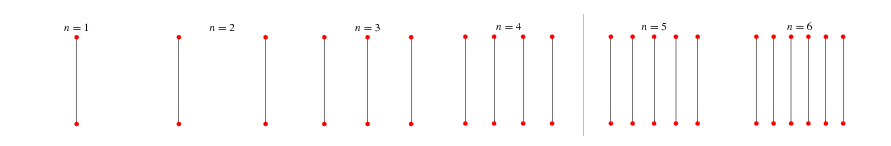
\includegraphics[scale=0.3]{img/disconnected.png} 
	  \end{figure}
	  
	  \begin{figure}
	    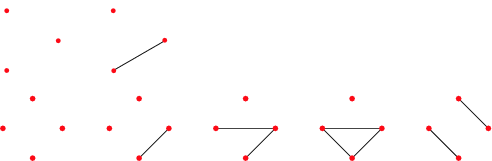
\includegraphics[scale=0.3]{img/disconnected_2.png} 
	  \end{figure}
\end{block}

\pause

\begin{block}{Componentes conexas}
�Qu� pasa en general cuando tenemos varias componentes conexas? �C�mo impacta en el conjunto dominante?
\end{block}

\end{frame}

\begin{frame}{Algunas familias (3)}

\begin{block}{Grafo A}
	\begin{figure}
	    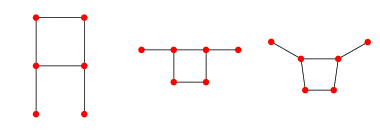
\includegraphics[scale=0.3]{img/AGraph.png} 
	  \end{figure}
\end{block}
\pause
\begin{block}{Coronas }
	\begin{figure}
	    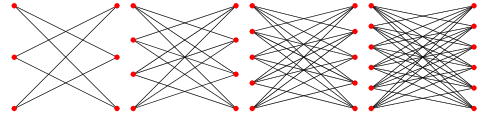
\includegraphics[scale=0.3]{img/crown_graphs.png} 
	  \end{figure}
\end{block}

Pueden encontrar muchas familias de grafos �tiles en los links de las referencias.

\end{frame}


%\begin{frame}{Heur�sticas constructivas greedy}
%\begin{block}{Ideas constructivas}
%	\begin{itemize}
%		\item \pause Nodo de mayor grado
%		\item \pause Nodo con mayor cantidad de vecinos a�n no dominados
%		
%	\end{itemize}
%\end{block}
%\end{frame}
%
%\begin{frame}{Heur�sticas de b�squeda local}
%\end{frame}

\begin{frame}
\begin{block}{Referencias}
	\begin{itemize}
		  \item Gross, L., \textit{Handbook of Graph Theory}. Chapter 9.2 - Domination in Graphs
		  
		  \item Information Systen on Graph Classes and their Inclusions, \url{http://www.graphclasses.org/smallgraphs.html}.
		  \item Wolfram MathWorld - Simple Graphs, \url{http://mathworld.wolfram.com/topics/SimpleGraphs.html}.
%		  \item \url{http://www.inf.usi.ch/kuhn/teaching/netalg/lectures/chapter7.pdf}
	\end{itemize}
\end{block}
\end{frame}

\end{document}
